\documentclass[a4paper,12pt]{article}
\usepackage[utf8]{inputenc}
\usepackage[T1]{fontenc}
\usepackage[spanish,es-sloppy]{babel}
\usepackage{listings}
\usepackage{xcolor}
\usepackage{amsmath}
\usepackage{graphicx}
\usepackage{here}
\usepackage{amsfonts}
\usepackage{amssymb}
\usepackage[left=2cm,right=1.5cm,top=1.5cm,bottom=1.5cm]{geometry}
\lstset{
language=C++,
backgroundcolor=\color{black!5},
frame=tb,
tabsize=4,
showstringspaces=false,
numbers=left,
commentstyle=\color{gray},
keywordstyle=\color{teal},
stringstyle=\color{orange},
basicstyle=\footnotesize}
\title{Standard Template Library \& Estructura de datos}
\author{HeNeos}
\begin{document}
\maketitle
\section{PC-UNI}
\subsection*{Objetivos}
\begin{enumerate}
\item Familiarizarse con la STL.
\item Ver problemas de fuerza bruta.
\end{enumerate}
\subsection*{STL (Standard Template Library)}
Básicamente podemos ver a la STL como una colección de una estructura de datos y funciones de uso común que nos hará la vida más sencilla. Esta librería es muy amplia, pero solo requerimos una pequeña parte de ella para Programación Competitiva y bastará con practicar regularmente con ella para poder implementar sin problemas soluciones que se nos ocurran a los problemas.
\subsubsection*{¿Qué tan frecuente la usaremos?}
Básicamente la usaremos siempre en nuestras soluciones.\\
Por ejemplo, es común que las soluciones que programemos tengan que hacer un ordenamiento como una subrutina en $O(n\log n)$, para lo cual podríamos implementar, por ejemplo el \textit{Merge Sort} o podríamos usar:
\begin{lstlisting}
std::sort() //1 linea. O(n log n).
\end{lstlisting}
\subsection*{¿Siempre que usemos algo de la STL tendremos que usar como prefijo `std::' y declarar una a una las librerías que usaremos?}
Depende de ti. Por ejemplo, si tuvieras que leer un número $n$ seguido de $n$ números; y tuvieras que imprimir los $n$ números ordenados podrias hacer una solución así:
\begin{lstlisting}
#include <iostream>
#include <vector>
#include <iterator>
#include <algorithm>

int main () {
  int n;
  std::cin >> n;
  std::vector <int> arr(n);
  for (int i = 0; i < n; i++) {
    std::cin >> arr[i];
  }
  std::sort(std::begin(arr), std::end(arr));
  for (int arr_i: arr) {
    std::cout << arr_i << ' ';
  }
  std::cout << std::endl;
  return (0);
}
\end{lstlisting} 
O también podrías hacer algo como esto:
\begin{lstlisting}
#include <bits/stdc++.h>
// Con esto nos evitamos estar incluyendo todas (para efectos de competitiva)
// las librerias que necesitemos

using namespace std;
// Cuando incluimos esto nos evitamos estar escribiendo ::std

int main () {
  int n;
  vector <int> arr(n);
  for (int i = 0; i < n; i++) {
    cin >> arr[i];
  }
  for (int arr_i: arr) {
    cout << arr[i] << ' ';
  }
  cout << endl;
  return (0);
}
\end{lstlisting}
\subsubsection*{Ahora si, veamos algunas estructuras de datos que nos brinda la STL,$\ldots$ pero que es una estructura de datos?}
Es la forma como guardamos-organizamos los datos (cada estructura de datos tiene sus ventajas y desventajas). Comencemos con las estructuas que más utilizaremos.
\subsection*{Vectores}
Imaginemos que tenemos $n$ dominos y queremos hacer una fila con ellos en nuestra sala. Además en cada dominó queremos pegar 1 papel encima donde escribamos la posición que ocupa el dominó en la fila (obviamente las posiciones comenzarán en 0) y en la cara frontal del dominó escribiremos el nombre de un Pokémon. Además, siempre estamos ubicados al final de la fila desde un ángulo en el que podemos ver los papeles con las posiciones de todos los dominós pero solo el nombre del último Pokémon de la fila.\\
Para hacer dicha tarea, nos interesaría hacer las siguientes acciones:
\begin{description}
\item[Agregar-Quitar un dómino al final de la fila.]\hfill \\ Como siempre estamos ubicados al final de la fila y esta actividad es bien básica. Podriamos decir que estas actividades tienen complejidad $O(1)$.
\item[Ver que Pokémon está en alguna posición dada.]\hfill \\ Como siempre podemos ver todos los papeles con las posiciones, no debería ser difícil encontrar la posición que buscamos y mover un poco nuestro ángulo para revisar que Pokemón esta en esa posición. Así, podriamos decir que esta actividad es $O(1)$.
\item[Ver en que posiciones está un Pokémon dado.]\hfill \\Como no sabemos como estan distribuidos los dominos. Lo más natural sería revisar el Pokemón escrito en cada ficha. Es decir, esto sería $O(n)$.
\item[Agregar-Eliminar un dominó en cualquier posición.] \hfill \\ Si agregamos-quitamos un domino en una posición, tendremos que actualizar las posiciones de todos los dominos delante de este. Ahora, en el peor de los casos (agregar-quitar un domino al inicio) tendríamos que actualizar todas las posiciones. Luego esta operación sería $O(n)$.
\item[Mover todos los dominós a un lado.]\hfill \\ Si, por ejemplo, queremos mover toda la fila más a la derecha, lo más natural y sencillo sería ir moviendo cada domino uno a uno. Así, dicha actividad la podríamos hacer en $O(n)$.
\end{description}
Y bien, básicamente un vector hace la anterior tarea donde los papeles de los dominos con las posiciones son los índices de los elementos del vector y los nombres de los Pokemones son los datos que guarda el vector.\\
En C++ la sintaxis de las anteriores acciones sería:
\begin{lstlisting}
#include <bits/stdc++.h>

using namespace std;

int main () {
  vector <int> arr;
  // Agregar un elemento al final - O(1)
  arr.push_back(123);
  arr.push_back(987);
  arr.push_back(343);
  arr.push_back(134);
  arr.push_back(345);
  // Quitar un elemnto del final - O(1)
  arr.pop_back();
  // Agregar un elemento en la posicion `i` - O(n)
  int i = 2;
  arr.insert(begin(arr) + i, 234);
  // Eliminar un elemento de la posicion `i` - O(n)
  i = 1;
  arr.erase(begin(arr) + i);
  // Copiar el vector - O(n)
  vector <int> arrCopy = arr;
  // Para iterar el arr podemos hacerlo asi:
  for (int arr_i: arr) ;
  // O tambien asi
  // arr.size() nos retorna la cantidad de elementos - O(1)
  for (int i = 0; i < arr.size(); i++) ;
  // Si queremos eliminar todos los elementos - O(n)
  arr.clear();
  return (0);
}
\end{lstlisting}
\begin{figure}[H]
\centering
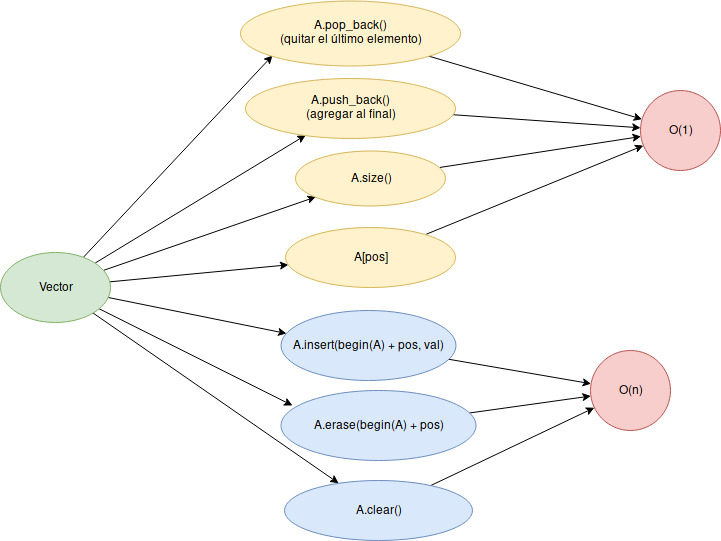
\includegraphics[scale=0.6]{vector}
\caption{En resumen, los métodos más frecuentes a usar en vectores}
\end{figure}
\subsection*{Deque}
Ahora, queremos una estructura que nos permita todo lo que un vector nos ofrece y 2 operaciones más:
\begin{itemize}
\item Insertar un elemento al inicio en $O(1)$.
\item Eliminar el primer elemento en $O(1)$.
\end{itemize}
\begin{lstlisting}
// La sintaxis es la misma que la de std::vector
// Pero ahora la declaracion es asi
deque <int> arr;
// ...
// Agregar un elemento al inicio - O(1)
arr.push_front(123);
// Eliminar el primer elemento - O(1)
arr.pop_front();
\end{lstlisting}
\subsubsection*{Algunas funciones útiles para vectores}
Antes de ver dichas funciones es bueno señalar que cuando una función de la STL require un rango como parámetros, siempre los recibe en esta forma: $[\mathtt{inicio}{,}\mathtt{fin})$. Así, por ejemplo, si quiero aplicar una función de la STL a los elementos de posiciones $[4{,}7]$ tendría que brindar los parámetros: $(\mathtt{begin(A)}+4{,}\mathtt{begin(A)}+8)$. Por ejemplo:
\begin{lstlisting}
vector <int> A = {12, 43, -13, 100, 100, -10};
// Busca el maximo elemento en todo el vector
cout << *max_element(begin(A), end(A)) << endl;
// Busca el maximo elemento en [0, 2]
cout << *max_element(begin(A), begin(A) + 3) << endl;
// Algunas de las funciones de la STL nos retornan punteros a elementos
// Por ejemplo la anterior funcion nos retorna un puntero al maximo elemento
// en el rango dado. Por ello, para acceder a su valor ponemos el `*' al
// inicio de la funcion
\end{lstlisting}
\subsubsection*{Otras funciones que podríamos usar}
\begin{description}
\item[\texttt{min\_element}] \hfill \\Devuelve un iterador que apunta al elemento con el valor más pequeño en el rango [\texttt{first}, \texttt{last}).
\begin{lstlisting}
vector <int> A = {12, 43, -13, 100, 100, -10};
// Busca el minimo elemento en todo el vector
cout << *min_element(begin(A), end(A)) << endl;
// Busca el minimo elemento en [0, 2]
cout << *min_element(begin(A), begin(A) + 3) << endl;
\end{lstlisting}
\item[\texttt{minmax}] \hfill \\ Devuelve un \texttt{pair} con el menor de \texttt{a} y \texttt{b} como primer elemento, y el mayor como segundo. Si ambos son iguales, la función devuelve \texttt{make\_pair(a,b)}.
\begin{lstlisting}
int main () {
  auto result = minmax({1,2,3,4,5});
  cout << "minmax({1,2,3,4,5}): ";
  cout << result.first << ', ' << result.second << '\n'; //Nos mostrara 1,5
  return 0;
}
\end{lstlisting}
\item[\texttt{sort}] \hfill \\ Ordena los elementos en el rango [\texttt{primero}, \texttt{último}) en orden ascendente.
\begin{lstlisting}
int main () {
  int myints[] = {32,71,12,45,26,80,53,33};
  vector<int> myvector (myints, myints+8);// 32 71 12 45 26 80 53 33
  sort (myvector.begin(), myvector.begin()+4);//(12 32 45 71)26 80 53 33
  sort (myvector.begin()+4, myvector.end());// 12 32 45 71(26 33 53 80)
  sort (myvector.begin(), myvector.end());//(12 26 32 33 45 53 71 80)
}
\end{lstlisting}
\item[\texttt{fill}] \hfill \\ Asigna \texttt{val} a todos los elementos en el rango [\texttt{primero},\texttt{último}).
\begin{lstlisting}
int main () {
  vector<int> myvector (8);                       // myvector: 0 0 0 0 0 0 0 0
  fill (myvector.begin(),myvector.begin()+4,5);   // myvector: 5 5 5 5 0 0 0 0
  fill (myvector.begin()+3,myvector.end()-2,8);   // myvector: 5 5 5 8 8 8 0 0
}
\end{lstlisting}
\item[\texttt{reverse}] \hfill \\Revierte el orden de los elementos en el rango [\texttt{first},\texttt{last}).
\begin{lstlisting}
int main () {
  vector<int> myvector;
  for (int i=1; i<10; ++i) myvector.push_back(i);   // 1 2 3 4 5 6 7 8 9
  	  reverse(myvector.begin(),myvector.end());    // 9 8 7 6 5 4 3 2 1
}
\end{lstlisting}
\item[\texttt{random\_shuffle}]\hfill \\Reorganiza los elementos en el rango [\texttt{primero},\texttt{último}) al azar.
\begin{lstlisting}
int main () {
  vector<int> myvector;
  for (int i=1; i<10; ++i) myvector.push_back(i); // 1 2 3 4 5 6 7 8 9
  random_shuffle ( myvector.begin(), myvector.end() );
}
\end{lstlisting}
\item[\texttt{count}] \hfill \\Retorna el número de elementos en el rango [\texttt{primero},\texttt{último}) que sean iguales a \texttt{val}.
\begin{lstlisting}
int main () {
  int myints[] = {10,20,30,30,20,10,10,20};   // 8 elements
  int mycount = count (myints, myints+8, 10);
  cout << "10 appears " << mycount << " times.\n";
  vector<int> myvector (myints, myints+8);
  mycount = std::count (myvector.begin(), myvector.end(), 20);
  cout << "20 appears " << mycount  << " times.\n";
  return 0;
}
\end{lstlisting}
\end{description}
Sin embargo, la STL no limita esas funciones solo a los vectores. Tambien puedes aplicar a deque y en realidad a una gran clase de estructuras (como iras viendo poco a poco).
\subsubsection*{¿Y qué pasa si quiero guardar algo distinto a \texttt{int} en un vector?}
\begin{lstlisting}
// vector <tipo de dato> arr;
// Por ejemplo
vector <double> arr1;
vector <long long> arr2;
vector <string> arr3;
vector <char> arr4;
// ...
\end{lstlisting}
\subsubsection*{¿y que hay si quiero guardar tipos de datos más complejos en un vector?}
Para ello podrías usar un \texttt{struct} o una \texttt{class}. Sin embargo, aún no veremos ello. Aunque podrás encontrar un poco de ello en la bibliografía.
\subsection*{Pairs}
Es bueno añadir que comunmente necesitaras guardar pares. Para ello puedes usar un \texttt{pair}. Así:
\begin{lstlisting}
// pair <tipo de dato 1, tipo de dato 2> p1;
// Por ejemplo
pair <int, int> p1;
cout << p1.first << ' ' << p1.second << endl;
pair <int, double> p2;
pair <string, long long> p3;
vector <pair <int, int>> arr;
// ...
\end{lstlisting}
\subsection*{Matrix}
\begin{lstlisting}
// Si queremos una matrix de n por m
int n = 10, m = 20;
vector <vector <int>> mat1;
for (int i = 0; i < n; i++) {
  vector <int> row;
  for (int j = 0; j < m; j++) row.push_back(0);
  mat1.push_back(row);
}
// Tambien puedes armar la matrix de n por m asi
vector <vector <int>> mat2;
for (int i = 0; i < n; i++) {
  vector <int> row(m, 0);
  mat2.push_back(row);
}
// O incluso Asi
vector <vector <int>> mat(n, vector <int> (m, 0));
\end{lstlisting}
\subsubsection*{¿Siempre debo usar la STL?}
Usala con criterio. Si ves que solo te esta complicando la vida y hay una forma mas sencilla (con la misma complejidad). Solo has lo que te parezca mas natural.
\subsection*{Set}
Esta estructura sería el analogo en programación de lo que un conjunto es en Matemática. Los elementos en un \texttt{Set} solo se consideran una vez (Por ejemplo, si ingresaramos 10 veces el numero 1 a un conjunto, este solo se consideraria una vez) y el orden de sus elementos no importa. Pues: \{1, 2, 3\} = \{3, 2, 1\}.\\
Aunque, en realidad, la implementacion de un \texttt{Set} en C++ internamente guarda los elementos en orden creciente por detalles internos. Las operaciones que maneja un \texttt{Set} son:
\begin{itemize}
\item Insertar (\texttt{val}) en $O(\log n)$
\item Encontrar (\texttt{val}) en $O(\log n)$
\item Eliminar (\texttt{val}) en $O(\log n)$
\item Mostrar la cantidad de elementos en O(1)
\end{itemize}
Veamos un poco la sintaxis:
\begin{lstlisting}
set <int> S;
// Insertar un elemento - O(log n)
S.insert(3);
S.insert(4);
S.insert(-100);
S.insert(-345);
// Comprobemos que los elementos son guardados en orden ascendente
for (auto x: S) {
  cout << x << endl;
}
// Ver si un elemento pertenece al Set - O(log n)
if (S.count(4) > 0) {
  cout << "4 esta en el Set\n";
}
// Tambien podemos usar find para esto
if (S.find(4) != end(S)) {
  cout << "4 esta en el Set" << endl;
}
// Eliminar un elemento - O(log n)
S.erase(4);
// Tambien podemos eliminar asi
S.erase(S.find(4));
// Si previamente guardamos
// auto it = S.find(val) - O(log n)
// Luego
// S.erase(it) - O(1)
\end{lstlisting}
\begin{figure}[H]
\centering
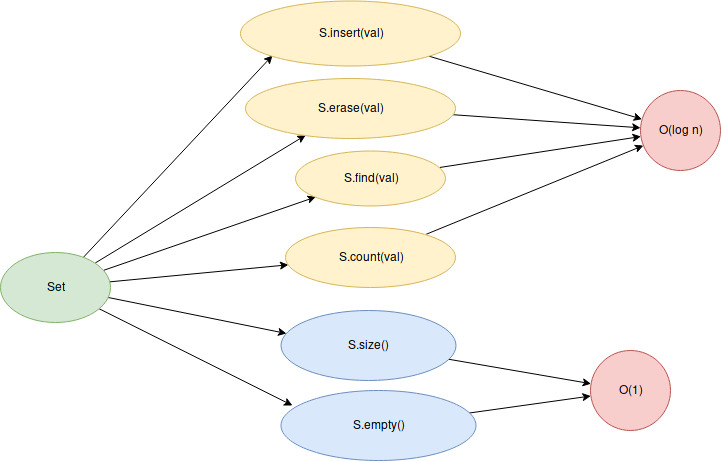
\includegraphics[scale=0.5]{set}
\end{figure}
\subsection*{MultiSet}
Un \texttt{MultiSet} tiene las funcionalidades de un \texttt{Set}, pero acepta duplicados de elementos.
\begin{lstlisting}
multiset <int> S;
// ...
int val = 3;
S.count(val); // Retornara cuantas veces `val` esta en el Multiset
// ...
S.erase(val); // Eliminara todas las ocurriencias de `val` en el Multiset
// ...
S.erase(S.find(val)); // Eliminara una ocurrencia de `val` del Multiset
\end{lstlisting}
\subsection*{Map}
Asi como un \texttt{Set} era una especie se analógo de lo que es un conjunto en Matemática para Computación. Un \texttt{Map} sería el análgo de lo que es una función en Matemática para Computación.
Es decir, un \texttt{Map} nos permite asociar tipos de datos. \texttt{Map <tipo 1, tipo2> mp;}\\
Analogo a una función en Matemática (donde $f(x) = y$ quiere decir que no existe un $y_{2}$ distinto de $y$ tal que 
$f(x) = y_{2}$).\\
Un \texttt{Map }solo tiene un valor asociado para un valor de tipo 1 (llamaremos clave o key a este). Es decir, un \texttt{Map} no tiene Keys iguales con distintos valores asociados.
\begin{lstlisting}
map <string, long long> mp1;
mp1["jose"] = 1000000;
mp1["leonidas"] = 42;
map <string, string> mp2;
mp2["hola"] = "mundo";
map <string, vector <string>> mp3;
map <pair <int, int>, int> mp4;
map <int, set <int>> mp5;
// ...
// Un Map tiene los mismos metodos de un Set y en si la misma complejidad
\end{lstlisting}
\subsection*{MultiMap}
Similar al \texttt{MultiSet}, un \texttt{MultiMap} es un \texttt{Map} que puede tener Keys iguales con distintos valores asociados.\\
Sim embargo, esta estructura casi no es utilizada en Competitiva.
\subsection*{Stacks}
Los \texttt{Stacks} (pilas) son un tipo de adaptadores de contenedor con el tipo de trabajo LIFO (Last In First Out), donde se agrega un nuevo elemento en un extremo y (arriba) un elemento se elimina solo de ese extremo. Las funciones asociadas con \texttt{Stack} son:
\begin{itemize}
\item \texttt{empty()} Retorna si el \texttt{Stack} está vacía - $O(1)$.
\item \texttt{size()} Retorna el tamaño del \texttt{Stack} - $O(1)$.
\item \texttt{top()} Retorna el elemento en la parte superior del \texttt{Stack} - $O(1)$.
\item \texttt{push(g)} Añade el elemento `g' a la parte superior del \texttt{Stack} - $O(1)$.
\item \texttt{pop()} Borra el elemento superior del \texttt{Stack} - $O(1)$.
\end{itemize}
\begin{lstlisting}
void showstack(stack <int> s) { 
    while (!s.empty()){ 
        cout << '\t' << s.top(); 
        s.pop(); 
    } 
    cout << '\n'; 
} 
  
int main (){ 
    stack <int> s; 
    s.push(10); 
    s.push(30); 
    s.push(20); 
    s.push(5); 
    s.push(1); 
    cout << "The stack is : ";
    showstack(s); //1  5  20  30  10
    cout << "\ns.size() : " << s.size(); // 5
    cout << "\ns.top() : " << s.top(); // 1
    cout << "\ns.pop() : ";
    s.pop(); 
    showstack(s); // 5  20  30  10
    return 0; 
} 
\end{lstlisting}
\subsection*{Queues}
Queues (colas) son un tipo de adaptadores de contenedor del tipo FIFO (First In First Out). Los elementos se insertan en la parte posterior (final) y se eliminan en la parte frontal.
\begin{itemize}
\item \texttt{empty().} Retorna si el \texttt{Queue} está vacía.
\item \texttt{size().} Retorna el tamaño del \texttt{Queue}.
\item \texttt{queue::swap() in C++ STL.} Intercambia el contenido de dos \texttt{Queue}, pero las \texttt{Queue} deben ser del mismo tipo, aunque los tamaños pueden ser diferentes.
\item \texttt{queue::emplace() in C++ STL.} Inserta un nuevo elemento en el contenedor del \texttt{Queue}, el nuevo elemento se agrega al final del \texttt{Queue}.
\item \texttt{queue::front() and queue::back in C++ STL.} La función \texttt{front()} devuelve una referencia al primer elemento del \texttt{Queue}. La función \texttt{back()} devuelve una referencia al último elemento de la \texttt{Queue}.
\item \texttt{push(g) and pop().} La función \texttt{push(g)} agrega el elemento 'g' al final del \texttt{Queue} y la función \texttt{pop()} elimina al primer elemento del \texttt{Queue}.
\end{itemize}
\begin{lstlisting}
void showq(queue <int> gq) { 
    queue <int> g = gq; 
    while (!g.empty()) 
    { 
        cout << '\t' << g.front(); 
        g.pop(); 
    } 
    cout << '\n'; 
}
int main() { 
    queue <int> gquiz; 
    gquiz.push(10); 
    gquiz.push(20); 
    gquiz.push(30); 
    cout << "The queue gquiz is : ";
    showq(gquiz); //10  20  30
    cout << "\ngquiz.size() : " << gquiz.size(); //3
    cout << "\ngquiz.front() : " << gquiz.front(); //10
    cout << "\ngquiz.back() : " << gquiz.back(); //30
    cout << "\ngquiz.pop() : ";
    gquiz.pop();
    showq(gquiz); //20  30
    return 0; 
} 
\end{lstlisting}
\subsection*{Priority Queue}
Un \texttt{Priority Queue} son un tipo de adaptadores de contenedor, diseñados específicamente para que el primer elemento del \texttt{Queue} sea el mayor de todos los elementos de la cola y los elementos estén en orden no decreciente (por lo tanto, podemos ver que cada elemento del \texttt{Queue} tiene un \texttt{priority\{fixed order\}}.
\begin{itemize}
\item \texttt{empty().} Retorna si el \texttt{Priority Queue} está vacío.
\item \texttt{size().} Retorna el tamaño del \texttt{Priority Queue}.
\item \texttt{top().} Retorna una referencia el elemento más arriba del \texttt{Priority Queue}.
\item \texttt{push(g).} Añade el elemento 'g' a el final del \texttt{Priority Queue}.
\item \texttt{pop().} Borra el primer elemento del \texttt{Priority Queue}.
\item \texttt{swap().} Intercambia el contenido de una \texttt{Priority Queue} con otra, pero deben ser del mismo tipo y tamaño.
\item \texttt{value\_type().} Representa el tipo de objeto almacenado como un elemento en un \texttt{Priority Queue}.
\end{itemize}
\section{TopCoder}
\subsection*{Containers}
Cada vez que necesite operar con muchos elementos, necesitará algún tipo de \texttt{Container}. En C nativo solo había un tipo de \texttt{Container}, el \texttt{array}.\\
El problema no es que los \texttt{arrays} sean limitados. El problema principal es que muchos problemas requieren un \texttt{Container} con mayor funcionalidad.\\
Por ejemplo, podemos necesitar una o más de las siguientes operaciones:
\begin{itemize}
\item Agregar alguna \texttt{string} a un \texttt{Container}.
\item Retirar una \texttt{string} de un \texttt{Container}.
\item Determinar si un \texttt{string} está presente en el \texttt{Container}.
\item Retornar el número de elementos distintos en un \texttt{Container}.
\item Iterar a través de un \texttt{Container} y obtener una lista de \texttt{strings} agregadas en algún orden.
\end{itemize}
Por supuesto, uno puede implementar esta funcionalidad en un \texttt{array} ordinario. Pero, la implementación trivial sería muy ineficiente. Puedes crear el \texttt{tree-of-hash-structure} para resolver esto de una forma rápida, pero piense un poco: ¿la implementación de dicho \texttt{container} depende los elementos que vamos a almacenar? ¿Tenemos que volver a implementar el módulo para hacerlo funcional, por ejemplo, para puntos en un plano pero no para \texttt{strings}. Si no, podemos desarrollar la interfaz para dicho \texttt{container} una vez, y luego usarla en cualquier lugar para datos de cualquier tipo. Esto, en definitiva, es la idea de los \texttt{containers} de la STL.
\subsection*{Antes de empezar}
Cuando el programa utiliza la STL, deberíamos \texttt{\#include} los encabezados estándar apropiados. Para la mayoría de los \texttt{containers}, el título del encabezado estándar coincide con el nombre del \texttt{container}, y no se requiere ninguna extensión. Por ejemplo, si va a usar el \texttt{stack}, simplemente agregue la siguiente línea al comienzo de su programa:
\begin{lstlisting}
#include<stack>
\end{lstlisting}
Los  tipos de \texttt{containers} (y los algoritmos, los \texttt{functors} y todo lo de la STL también) no son definidos en \texttt{global namespace}, pero si en el especial \texttt{namespace} llamado \texttt{"std"}. Añade la siguiente línea después de tus \texttt{include} y antes de empezar el código:
\begin{lstlisting}
using namespace std;
\end{lstlisting} 
Otra cosa importante a recordar es que el tipo de \texttt{container} es un \texttt{template} del parámetro. Los \texttt{template} del parámetro se especifican con \texttt{"</>"}. Por ejemplo:
\begin{lstlisting}
vector <int> N;
\end{lstlisting}
Al realizar construcciones anidadas, asegúrese de que los \textit{corchetes} no se están siguiendo directamente, deje un espacio en blanco entre ellos:
\begin{lstlisting}
vector <vector <int> >; //Correct Definition
\end{lstlisting}
\subsection*{Vector}
El \texttt{Container} STL más simple es \texttt{vector}. \texttt{Vector} es un \texttt{array} con funcionalidad extendida. Por cierto, \texttt{vector} es el único \texttt{container} que es compatible con versiones anteriores al código C nativo.
\begin{lstlisting}
vector< int > v(10);
for(int i = 0; i < 10; i++) {
v[i] = (i+1)*(i+1);
}
for(int i = 9; i > 0; i--) {
v[i] -= v[i-1];
}
\end{lstlisting}
Cuando escribimos:
\begin{lstlisting}
vector <int> v;
\end{lstlisting}
Se crea un vector vacío. Tenga cuidado con las construcciones como:
\begin{lstlisting}
vector <int> v[10];
\end{lstlisting}
Aquí declaramos 'v' como un \texttt{array} de 10 \texttt{vector <int>}, que inicialmente están vacías. En la mayoría de los casos, esto no es lo que queremos. Use paréntesis en lugar de corchetes. La característica más utilizada de un \texttt{vector} es que puede retornar su tamaño.
\begin{lstlisting}
int elements_count = v.size();
\end{lstlisting}
\texttt{sie()} es \texttt{unsigned}, lo que a veces puede causar problemas. Por tanto, generalmente definimos macros como \texttt{sz(C)} que retorna el tamaño de \texttt{C} como un entero ordinario con signo. No es buena práctica comparar \texttt{v.size()} a 0 para saber si está vacío. Es mejor usar la función \texttt{empty()}.
\begin{lstlisting}
bool is_nonempty_notgood = (v.size() >= 0); // Try to avoid this
bool is_nonempty_ok = !v.empty();
\end{lstlisting}
Esto es porque no todos los \texttt{containers} pueden retornar su tamaño en tiempo $O(1)$.\\
Otra función muy popular para usar en vectores es \texttt{push\_back()}, la cual agrega un elemento al final del vector, aumentando su tamaño en uno. Considere el siguiente ejemplo:
\begin{lstlisting}
vector <int> v;
for(int i = 1; i < 1000000; i *= 2) {
v.push_back(i);
}
int elements_count = v.size();
\end{lstlisting}
No te preocupes por la asignación de memoria: \texttt{vector} no asignará un elemento cada vez, en su lugar, el vector asigna más memoria que la que realmente necesita cuando se agregan nuevos elementos con \texttt{push\_back}. Cuando necesitamos cambiar el tamaño de un vector podemos usar la función \texttt{resize()}. La función \texttt{resize()} hacer que \texttt{vector} contenga el número requerido de elementos. Si necesita menos elementos de los que ya contiene, entonces los últimos serán eliminados. Si le pide al \texttt{vector} que crezca, aumentará su tamaño y llenará con ceros los nuevos elementos creados. Tenga en cuenta que si utiliza \texttt{push\_back()} después de usar \texttt{resize()}, agregará los elementos después del tamaño asignado, pero no en ellos:
\begin{lstlisting}
 vector< int > v(20);
for(int i = 0; i < 20; i++) {
v[i] = i+1;
}
v.resize(25);
for(int i = 20; i < 25; i++) {
v.push_back(i*2); // Writes to elements with indices [25..30), not [20..25) ! <
}
\end{lstlisting}
Para limpiar un \texttt{vector} podemos usar la función \texttt{clear()}. Esta función hace que el \texttt{vector} contenga 0 elementos. No hace que los elementos sean 0's, borra completamente al \texttt{vector}.\\
Hay muchas formar de inicializar un vector:
\begin{lstlisting}
vector< int > v1;
// ...
vector< int > v2 = v1;
vector< int > v3(v1);
\end{lstlisting}
La inicialización de 'v2' y 'v3' son iguales. Si tu quieres crear un \texttt{vector} con un tamaño especificado, puedes usar el siguiente constructor:
\begin{lstlisting}
vector <int> Data(1000);
\end{lstlisting}
En el ejemplo arriba, el \texttt{Data} contiene 1000 ceros después de su creación. Recuerde usar paréntesis y no corchetes. Si quieres que el \texttt{vector} se inicialize con otra cosa, escríbalo de tal forma:
\begin{lstlisting}
vector <string> names(20, "Unknown");
\end{lstlisting}
Recuerde que puedes crear un \texttt{vector} de cualquier tipo. \texttt{Arrays} multidimensionales son muy importantes, la manera más simple de crear un \texttt{array} \texttt{bi-dimensional} es crear un \texttt{vector} de \texttt{vectores}.
\begin{lstlisting}
vector <vector <int> > Matrix;
\end{lstlisting} 
\subsection*{Pairs}
Antes de llegar a los iteradores, permítame decir algunas palabras sobre los \texttt{pairs}. Los \texttt{pairs} son ampliamente utilizados en STL. Los problemas simples por lo general requieren una estructura de datos simple que se ajuste bien al \texttt{pair}. En general, el \texttt{pair <int, int>} es un \texttt{pair} de valores enteros. En un nivel más complejo, \texttt{pair <string, pair <int, int> >} es un \texttt{pair} de \texttt{string} y dos \texttt{int}.
\begin{lstlisting}
pair<string, pair< int,int > > P;
string s = P.first; // extract string
int x = P.second.first; // extract first int
int y = P.second.second; // extract second int
\end{lstlisting}
La gran ventaja de los \texttt{pairs} es que tienen operaciones integradas para compararse. Los \texttt{pairs} se comparan del elemento primero a segundo. Si los primeros elementos no son iguales, el resultado se basará solo en la comparación de los primeros elementos; los segundos elementos serán comparados solo si los primeros son iguales. El \texttt{array} de \texttt{pairs} se puede ordenar fácilmente por las funciones internas de la STL.\\
Por ejemplo, si deseamos ordenar un \texttt{array} de puntos enteros para que formen un polígono, es una buena idea colocarlos en el \texttt{vector <pair <double, pair <int, int> > >}, donde cada elemento del \texttt{vector} es \texttt{\{angulo, \{x, y\} \}}. Una llamada a la función de \texttt{sorting} de la STL le dará el orden de puntos deseado. Los \texttt{pairs} también se usan ampliamente en \texttt{containers} asociativos, de los que hablaremos más adelante en este artículo.
\subsection*{Iterators}
\textbf{¿Qué son los iteradores?} En STL, los \texttt{iterators} son la forma más general de acceder a los datos en \texttt{containers}. Considere el problema simple: Invierta el \texttt{array} A de N \texttt{int}:
\begin{lstlisting}
void reverse_array_simple(int *A, int N) {
int first = 0, last = N-1; // First and last indices of elements to be swapped
While(first < last) { // Loop while there is something to swap
swap(A[first], A[last]); // swap(a,b) is the standard STL function
first++; // Move first index forward
last--; // Move last index back
}
}
\end{lstlisting}
Este código debe ser claro para usted.
\begin{lstlisting}
#define all(c) c.begin(), c.end()
vector< int > X; 
// ... 
sort(X.begin(), X.end()); // Sort array in ascending order
sort(all(X)); // Sort array in ascending order, use our #define
sort(X.rbegin(), X.rend());//Ordena el array en orden decreciente
\end{lstlisting}
\end{document}
